\documentclass[UTF8,a4paper,11pt,fontset=none]{ctexart}
\usepackage[margin=25mm]{geometry}
\setmainfont{TeX Gyre Termes}
\setsansfont{TeX Gyre Heros}
\setmonofont{TeX Gyre Cursor}
\setCJKmainfont[ItalicFont={Noto Serif CJK SC},SlantedFont={Noto Serif CJK SC}]{Noto Serif CJK SC}
\setCJKsansfont{Noto Sans CJK SC}
\setCJKmonofont{Noto Sans Mono CJK SC}
\usepackage{graphicx}
\usepackage{amsmath,amssymb,booktabs}
\usepackage{natbib}
\usepackage{caption}
\usepackage{placeins}
\usepackage[hidelinks]{hyperref}
\captionsetup{font=small,labelfont=normalfont,labelsep=quad}
\hypersetup{pdfauthor={},pdftitle={知识蒸馏何时能够迁移？——来自热启动语言建模的受控实证证据}}
\setlength{\parindent}{2em}
\setlength{\parskip}{0pt}
\setlength{\emergencystretch}{2em}
% Keep inline equations, especially mean +/- SD quantities, on one line.
\binoppenalty=10000
\relpenalty=10000
\ctexset{section={format=\Large\bfseries,number=\arabic{section}},subsection={format=\large\bfseries}}
\title{知识蒸馏何时能够迁移？\\——来自热启动语言建模的受控实证证据\\[0.5em]
  {\large When Does Knowledge Distillation Transfer?\\Controlled Evidence from Warm-Start Language Modeling}}
\author{作者：课题组内部留档}
\date{}

\begin{document}
\maketitle
\begin{abstract}
知识蒸馏（KD）通常以蒸馏后学生模型的性能来评估，但一个基本问题仍未得到回答：对于一个已经训练过的学生模型，教师监督能否优于从相同状态出发的最大似然续训？我们通过匹配热启动续训、受控教师干预和独立学生模型重复实验，研究自回归语言建模中的这一问题。在相同的按词元归一化的形式下，KD 在 Penn Treebank 和 WikiText-2 上产生正迁移，在 TinyStories 上产生负迁移，且每种配置下的三个独立学生初始化均呈现一致方向。我们检验了几种可能的解释。在固定教师架构和融合组成的条件下，改变训练后的教师模型状态会逆转迁移方向，表明教师模型状态和预测质量会明显影响蒸馏。然而，教师模型的全局似然不足以解释迁移：一个留出集似然比匹配 CE 对照更差的教师模型，仍能改善全部三个学生模型。更大的分支分歧度和架构异质性并不意味着更好的迁移；在全部三组比较中，同构 Transformer 集成都优于异构 Transformer--Grassmann 教师。所检验的局部梯度和曲率诊断指标也未能可靠地预测长程迁移。综合来看，这些结果支持以匹配 CE 续训为对照，对热启动 KD 进行配置依赖的评估，而不是根据教师似然排序或所检验的局部诊断指标推断迁移。
\end{abstract}

\section{引言}\label{sec:introduction}

知识蒸馏（KD）将教师模型的预测信息迁移给较小的学生模型。自回归语言模型蒸馏目前已涵盖替代散度、同策略训练、自适应监督和教师选择。这些进展表明，更强的教师模型并不必然产生更强的学生模型。在选择更复杂的算法之前，一个实际问题需要先得到回答：对于一个已经训练过的学生模型，冻结教师监督能否优于从完全相同的状态出发的最大似然续训？

\begin{figure}[!t]
\centering
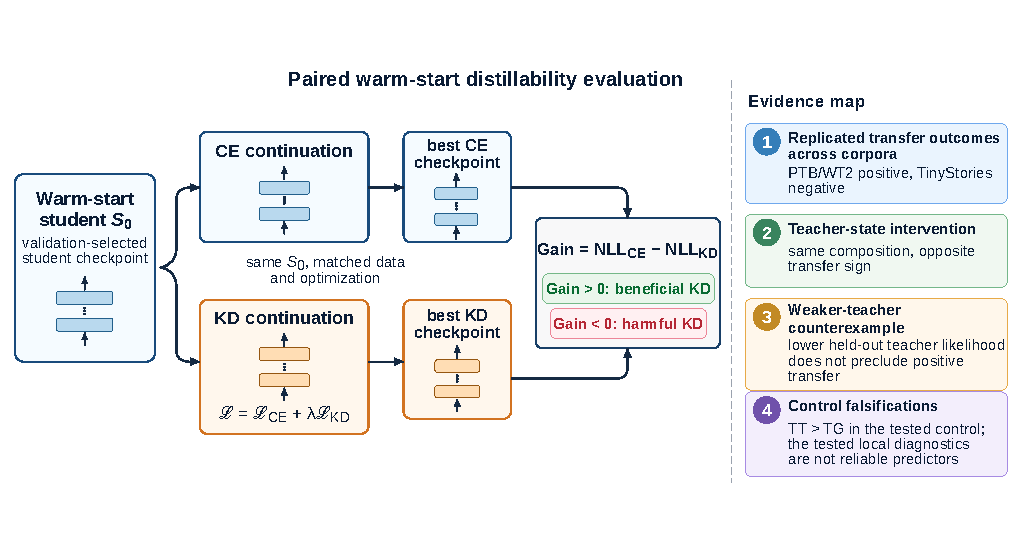
\includegraphics[width=\textwidth]{figures/fig1_paired_protocol.pdf}
\caption{配对热启动评估。完全相同的 $S_0$ 权重分别初始化 CE 和 KD；两者独立地基于验证集选择检查点，随后报告测试集结果。证据图将重复验证的迁移结果与解释范围受限的对照区分开来。}
\label{fig:paired_protocol}
\end{figure}

我们通过配对热启动评估研究这一问题。基于验证集选择的学生检查点 $S_0$ 同时初始化交叉熵（CE）续训和 KD 续训。两条实验路径均使用重新初始化的优化器，匹配续训数据和预算，然后独立地依据验证集似然选择检查点。两者的测试集 NLL 差值衡量的是在 CE 之外加入监督的价值，而不是相对于无关基线的改进。每项确认性比较均使用三个独立训练的学生初始化。

这一设计在相同的按词元归一化的 KD 形式下，揭示了可复现的正迁移和负迁移。PTB 和 WikiText-2 上的平均增益分别为 $0.1449$ 和 $0.1557$ NLL，而 TinyStories 上的性能退化幅度为 $0.1072$。每个领域的全部三个学生模型均呈现相同方向。这些结果并未确立语料身份的因果效应，因为各配置的教师模型、数据量和准备历史有所不同。因此，我们通过更受控的比较检验可能的解释。

教师质量是一项重要但不完整的解释。在固定 WikiText-2 教师架构、教师源身份和融合组成的条件下，联合训练的教师模型改善了全部三个学生模型，而仅训练融合权重的状态损害了全部三个学生模型。配对对比为 $0.1833$ NLL。教师训练状态及其产生的预测质量会明显影响迁移，但这一干预并未将标量似然单独识别为原因。相反，一个留出集似然比每个匹配的、基于验证集选择的 CE 对照都更差的 Grassmann-only 教师源，仍然改善了全部三个学生模型。因此，教师模型相对于匹配 CE 对照的似然优势并不是正迁移的必要条件。

在固定的 Transformer--Grassmann 检查点内，融合监督比任一单独分支的迁移效果更好。然而，同构 Transformer--Transformer 对照在全部三个学生模型上均取得了更好的 KD 终点，尽管其分支分歧度更低。教师质量、参数量和训练历史的差异，使我们无法将这一排序归因于架构。这一对照不支持 Grassmann 表征具有独特可迁移性，也不支持异构监督更优的主张。

回顾性的局部梯度和曲率分数也错误分类了若干在终点评估中稳定呈现正迁移的配置。我们将这些失败视为解释范围受限的证伪证据，而不是新的预测器或普遍的不可能性结论。所检验的统计量不能概括漫长的优化轨迹和基于验证集的选择。

本文的贡献是一条受控实证证据链：相对于配对 CE 对照的正迁移和负迁移、固定融合组成下的教师模型状态干预与迁移方向逆转、较弱教师源的反例、同构集成证伪对照，以及回顾性局部诊断指标的失败。我们不提出新的 KD 算法，也不声称首次发现有害 KD 或弱教师 KD。其实际意义在于，应当从所关注的学生状态出发，以匹配续训为对照评估教师监督，而不是根据单一的教师质量、多样性或局部兼容性统计量推断其价值。

\section{相关工作}\label{sec:related-work}

\subsection{教师质量与面向学生的监督}
KD 传递的是预测分布，而不仅是硬标签~\citep{hinton2015distilling}。模型容量不匹配以及训练后期有害的监督，已经表明教师质量与教学效用并不相同~\citep{cho2019efficacy}；学生友好型教师通过引入学生分支来应对这种不匹配~\citep{park2021friendly}。统计分析强调概率估计与偏差--方差权衡~\citep{menon2021statistical}，而表现较差的分类器在特定假设下也可以成为有效的教师~\citep{kaplun2022bad}。我们的贡献不是再次指出教师准确率可能不足以判断教学效用这一一般现象，而是构建受控的热启动 LM 实验证据链。

\subsection{自回归 LM 蒸馏}
MiniLLM 使用反向 KL 和策略梯度优化~\citep{gu2024minillm}；GKD 使用由学生生成的上下文，并允许采用不同的散度~\citep{agarwal2024gkd}。ATKD 针对容易和困难的词元调整监督~\citep{zhong2024atkd}，选择性 NMT 蒸馏则识别可能有害的指导信号~\citep{wang2021selective}。蒸馏缩放定律将学生似然与教师性能、模型规模及计算量联系起来~\citep{busbridge2025scaling}。相比之下，我们固定基于语料的正向 KL 续训方式，并从同一学生出发，评估相对于 CE 续训的增益。本研究不比较生成质量，也不证明优于这些方法。

\subsection{自适应监督、集成监督与梯度驱动的监督}
多教师选择~\citep{yuan2021selection}以及 MetaDistil 中基于学生测验集的反馈~\citep{zhou2022metadistil}，用于应对教师适配性问题。集成保真度与泛化能力并不等同~\citep{stanton2021really}；自适应集成 KD 则利用梯度协调相互竞争的指导信号~\citep{du2020agree}。AdaKD 自适应调整词元的关注程度与温度~\citep{xie2026adakd}；熵感知的同策略 KD 在不确定的词元上加入正向 KL~\citep{jin2026entropy}。GRACE 利用学生在教师生成回复上的梯度谱统计量对教师排序~\citep{panigrahi2026grace}，这与我们基于固定 logits 的验证集梯度探测不同。该工作还报告，在生成式教师选择中，验证集影响度基线的表现较弱；我们的探测则针对基于语料似然、相对于 CE 续训的配对终点。我们不评估这些自适应算法。本研究的对照实验与未成功的局部诊断分析补充了这一研究方向，但不提出新的兼容性理论。

\section{配对热启动评估}\label{sec:problem-setting}

对于每个独立准备的学生，使用按验证集选择的 $S_0$ 初始化 CE 和 CE+KD 两个分支，使二者具有相同的权重，并重新初始化优化器状态。续训数据、顺序、优化器、调度器与训练预算均保持匹配。每个分支独立依据验证集 NLL 选择检查点，并在选择完成后报告测试结果（图~\ref{fig:paired_protocol}）。

令 $p_{\mathrm{teach},i}^{(\tau)}$ 和 $p_{\mathrm{stud},i}^{(\tau)}$ 分别表示温度 $\tau$ 下的下一词元分布。在因果移位后的有效目标位置 $\mathcal I$ 上，目标函数为
\begin{align}
\mathcal L&=\mathcal L_{\mathrm{CE}}+\lambda\mathcal L_{\mathrm{distill}},\label{eq:kd-objective}\\
\mathcal L_{\mathrm{distill}}&=\frac{\tau^2}{|\mathcal I|}\sum_{i\in\mathcal I}
\mathrm{KL}\!\left(p_{\mathrm{teach},i}^{(\tau)}\|p_{\mathrm{stud},i}^{(\tau)}\right).\nonumber
\end{align}
两个损失都对目标词元求平均。主要 KD 实验固定 $\tau=2$ 和 $\lambda=5$；CE 使用 $\lambda=0$。用于实际比较的配对终点指标定义为
\begin{equation}
\mathrm{Gain}_{\mathrm{KD}}=\mathrm{NLL}_{\mathrm{CE}}^{\mathrm{test}}-\mathrm{NLL}_{\mathrm{KD}}^{\mathrm{test}}.
\label{eq:paired-gain}
\end{equation}
增益为正表示 KD 优于 CE，但不一定优于 $S_0$。这是特定实验协议下的终点指标，而非可蒸馏性的理论度量。

我们报告种子 42、123 和 456 的结果，以及配对增益均值、样本 SD 和符号一致性。这些种子改变的是学生准备过程，而不是教师训练或语料采样；SD 既不是标准误，也不能作为显著性检验。主要结果从已训练的续训检查点中进行选择。另一项单独标明的诊断分析允许将未修改的 $S_0$ 作为第 0 步候选，但不替代主要终点。

\section{实验设置与受控干预}\label{sec:experimental-setting}

主要语料为 PTB~\citep{marcus1993ptb}、WikiText-2~\citep{merity2016wikitext}和 TinyStories~\citep{eldan2023tinystories}。具有 31.43M 参数的 Transformer--Grassmann 混合学生使用本地 GPT-2 分词器，序列长度为 256，准备阶段的训练轮次为 20。匹配的续训为 10 个训练轮次，使用 AdamW，学习率为 $10^{-4}$，批大小为 32，权重衰减为 0.01，采用 5\% 预热与余弦衰减、AMP，以及阈值为 1 的梯度裁剪。不同语料采用的教师与准备历史不同；跨领域的绝对 NLL 不能直接比较。附录~\ref{app:architecture}和~\ref{app:protocols}给出复现细节。

异构实验平台中的教师通过 logits 层面的后融合，将 Transformer~\citep{vaswani2017attention}分支与因果 Grassmann 分支结合：
\begin{equation}
z_{\mathrm{TG}}=\alpha z^{(\mathrm T)}+(1-\alpha)z^{(\mathrm G)}.
\label{eq:teacher-fusion}
\end{equation}
该架构用于提供监督信号，而不是新的方法贡献。WikiText-2 状态干预比较联合训练的 J 与仅训练融合权重的 A，二者采用同一组源模型，并在使用时固定 $\alpha=0.5$。监督源消融固定 J，分别使用 $\alpha=0.5,1,0$，对应融合（F/TG）、仅 Transformer（T）和仅 Grassmann（G）监督。

同构 TT 对照增加一个独立准备的 Transformer，其源模型架构、数据、分词器及 20 个训练轮次的预算均相同。随后，TT 按 10 个训练轮次的联合教师训练计划进行训练，并在第 1 个训练轮次冻结分支；TT 与 TG 在使用时都设为 $\alpha=0.5$。它们完整的训练历史、融合学习率、参数量与预测质量并不相同。

教师模型状态与监督源的似然使用同一个包含 512 个数据块的验证子集（130,560 个目标）；TT/TG 使用完整验证集。这些评估范围保持区分。WikiText-2 对照复用 CE 和 TG 终点，不构成额外的独立重复实验。回顾性的局部诊断分析以及基于预训练 SmolLM2/FineWeb-Edu 的压力测试，与主要实验矩阵分开报告。

\section{正迁移与负迁移}\label{sec:cross-domain-transfer}

相同的词元归一化形式在 PTB 和 WikiText-2 上产生正迁移，在 TinyStories 上产生负迁移（表~\ref{tab:cross_domain_transfer}；图~\ref{fig:cross_domain_gain}）。每个领域的三个独立学生准备结果都具有一致的增益方向。在 TinyStories 上，CE 在全部三个种子中都优于 $S_0$，因此有害的 KD 是相对于有效的续训而言，而不是两个无需进行的训练分支之间的比较。

这些结果确立了所测试配置下的可重复性，但不构成语料效应的因果证据。不同领域的教师、数据量与学生准备过程不同。纳入分析的终点均为有限值；梯度裁剪与偶发的 AMP 更新跳过仍限制了从优化角度进行解释（附录~\ref{app:protocols}）。完整的终点 NLL 与各种子的增益见附录~\ref{app:per-seed}。

\begin{table}[t]
\centering
\begin{tabular}{lrr}
\toprule
数据集 & 增益（均值 $\pm$ 标准差） & 符号一致性\\
\midrule
PTB & $+0.144937\pm0.003938$ & 3/3 $+$\\
WikiText-2 & $+0.155665\pm0.007692$ & 3/3 $+$\\
TinyStories & $-0.107219\pm0.000415$ & 3/3 $-$\\
\bottomrule
\end{tabular}
\caption{每个语料上三个独立学生模型的配对测试集 NLL 增益；报告样本标准差，$\lambda=5$，$\tau=2$。两个分支均按验证集 NLL 选择检查点。}
\label{tab:cross_domain_transfer}
\end{table}

\begin{figure*}[!t]
\centering
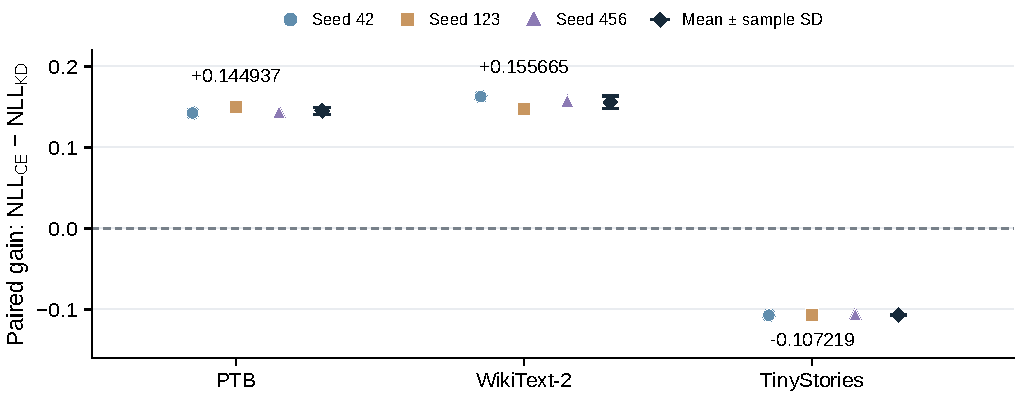
\includegraphics[width=\textwidth]{figures/fig2_cross_domain_gain.pdf}
\caption{相对于 CE 的测试 NLL 迁移结果。各散点表示独立的学生种子；黑色标记与误差条表示均值及样本 SD。正值表示 KD 更优。每个语料内部的教师与数据划分保持固定。}
\label{fig:cross_domain_gain}
\end{figure*}

\section{什么决定可蒸馏性？}\label{sec:distillability}

\subsection{固定组成下的教师模型状态与迁移反转}
\label{sec:teacher-state}
在相同的 $\alpha=0.5$ 下，联合训练的教师模型 J 在验证子集上的 NLL 为 4.300644，而仅训练融合权重的 A 为 6.376220。J 使全部三个学生的 NLL 改善 $+0.155665\pm0.007692$，而 A 使全部三个学生退化，增益为 $-0.027654\pm0.006822$。配对状态差异定义为
\begin{equation}
Q=\mathrm{NLL}_{\mathrm{KD,A}}-\mathrm{NLL}_{\mathrm{KD,J}},
\label{eq:teacher-state-contrast}
\end{equation}
其均值为 $+0.183319\pm0.001375$，在全部三个种子中均为正。

在固定架构与组成下，教师模型的训练状态及其形成的预测质量对迁移有较大影响。这不意味着标量似然具有因果作用：联合训练也改变表征与错误分布，而且教师训练预算不同。附录~\ref{app:protocols}保留了原始训练模式与训练准入条件的修订记录。

\subsection{较弱的监督源仍可产生正迁移}
\label{sec:weaker-teacher}
仅 Grassmann 的监督源在验证子集上的 NLL 为 4.652064，差于该子集上每一个匹配的、按验证集选择的 CE 对照模型。尽管如此，全部三个学生都得到改善，平均测试增益为 $+0.040991\pm0.006733$。对照是所选的 CE 续训模型，而非任意初始化模型。教师似然与匹配的 CE 终点在同一验证子集上比较，而迁移增益使用所选的测试终点进行评估（附录~\ref{app:per-seed}）。

这些对照共同表明，教师质量有较大影响，但全局留出集似然本身不足以判断监督是否有用。它们既不意味着教师质量无关紧要，也不将正迁移归因于几何结构（图~\ref{fig:teacher_quality}）。

\begin{figure}[!t]
\centering
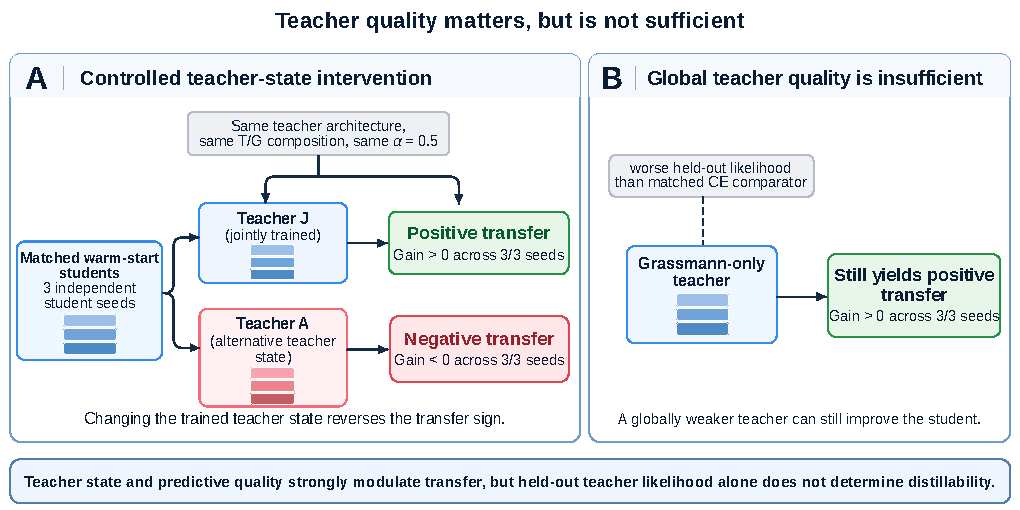
\includegraphics[width=\textwidth]{figures/fig3_teacher_quality.pdf}
\caption{WikiText-2 的状态与似然对照。在固定组成下，改变已训练的教师模型状态会反转迁移符号；似然差于 CE 的监督源仍能产生正迁移。这两项结果均不证明标量似然的因果作用或几何结构带来的 KD 优势。}
\label{fig:teacher_quality}
\end{figure}

\section{监督来源、集成与诊断对照}\label{sec:controls}

\subsection{融合监督与分支监督}
\label{sec:source-ablation}
固定 J 时，F、T 和 G 的平均增益分别为 $+0.155665$、$+0.134868$ 和 $+0.040991$。F 相对 T 的优势为 $+0.020797\pm0.001214$，相对 G 的优势为 $+0.114674\pm0.001001$，两组差异在全部三个种子上均为正。融合组成与预测质量同时发生变化，因此该对照不能单独确定融合收益的来源。

仅使用 T 的监督条件在资格门控阶段和首个正式训练轮次中，每次更新都会触发梯度裁剪，尽管参数梯度均为有限值。获准继续进行的续训保留了 \texttt{CLIP\_SATURATION\_WARNING}。应谨慎解释较小的 F--T 差距；附录~\ref{app:protocols} 记录了保持不变的训练协议与裁剪轨迹。

\subsection{同构集成证伪对照}
\label{sec:homogeneous-control}
TT 的增益为 $+0.168125\pm0.008948$，TG 的增益为 $+0.155665\pm0.007692$。配对差异定义为
\begin{equation}
H=\mathrm{Gain}_{\mathrm{TG}}-\mathrm{Gain}_{\mathrm{TT}}
=\mathrm{NLL}_{\mathrm{TT}}-\mathrm{NLL}_{\mathrm{TG}},
\label{eq:ensemble-contrast}
\end{equation}
其均值为 $-0.012460\pm0.001348$，全部三个差异均为负。在所测试的设置中，TG 教师模型相较于 TT 没有优势（图~\ref{fig:ensemble_control}）。

TT 教师模型在完整验证集上的 NLL 还低 0.010108，参数量约少 6.38\%，且融合权重学习率与训练历程均不同。这些混杂因素使得该排序不能归因于 TT 的内在优势。TG 的分支分歧更大，但 KD 增益并未更大；预测多样性不一定是可迁移的多样性。该比较不支持 Grassmann 特有优势或异构监督优势。

\subsection{局部诊断指标不能区分最终结果}
\label{sec:local-diagnostics}
在七个教师模型--领域组合、每个组合三个学生种子的回顾性分析中，一阶与二阶评分的 AUROC 均约为 0.644，符号准确率均约为 0.571。曲率没有增加符号区分能力，且这些评分将已知具有正向结果的 WikiText-2 组合判错。所测试的局部诊断指标不能可靠地预测这些最终结果。

一些标量预测指标对合并结果的区分能力更强，但这一规模较小且存在依赖关系的结果集合不能确立一般性的选择规则。在 CE 难度之外，词元级分支 JSD 增加的信息很少。附录~\ref{app:diagnostics-modern} 报告了完整指标、校准不稳定性及观察性分析的局限。这些失败涉及所测试的离线评分，不能推广到一般的自适应 KD 方法。

\begin{figure}[!t]
\centering
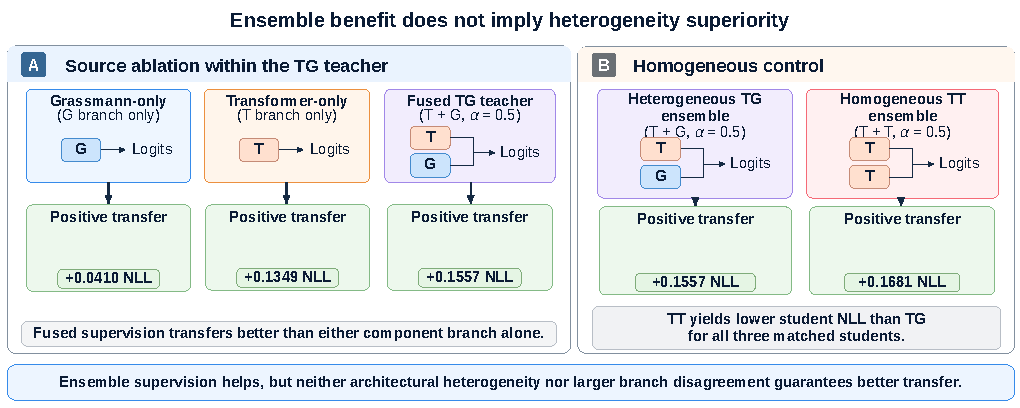
\includegraphics[width=\textwidth]{figures/fig4_ensemble_control.pdf}
\caption{WikiText-2 教师监督来源与集成的增益，保留四位小数。TT 在全部三个学生上均优于 TG。仅使用 T 的监督条件：早期裁剪饱和，应谨慎解释 F--T 差距。TT 与 TG 教师模型并非严格的质量匹配或训练匹配对照。}
\label{fig:ensemble_control}
\end{figure}

\section{外部有效性压力测试}\label{sec:external-validity}

在固定的 FineWeb-Edu 子集上~\citep{penedo2024fineweb}，一个完成适配后冻结的 SmolLM2-360M 教师模型为三个独立适配的 SmolLM2-135M 学生模型提供监督~\citep{benallal2025smollm2}。增益分别为 $-0.013550\pm0.003542$（$\lambda=1$）与 $-0.043924\pm0.004017$（$\lambda=5$）。尽管教师模型的似然更好，两种条件下均为 3/3 负向，且验证集与测试集上的方向一致。

然而，允许将 $S_0$ 作为第 0 步的验证候选后，全部九个 CE/KD 续训均选择 $S_0$。这一诊断不会替代以训练后检查点为候选的主要最终结果；它表明在该设置中，进一步 CE 续训本身已无必要。KD5 保留 \texttt{CLIP\_SATURATION\_WARNING}；KD1 也频繁触发裁剪。上述两项观察均不能证明裁剪是性能下降的原因。

一个仅使用 CE 的续训改进空间对照采用固定的早期学生检查点以及不重叠的额外目标词元。其最佳验证集改进为 $+0.004849$，未达到预注册的 0.01 门槛。因此，没有进行以门槛通过为前提的 KD 训练，也没有开展新的测试集评估。这些结果仍是限定范围的压力测试，不能视为对现代模型规模下有害 KD 的清晰确认（附录~\ref{app:diagnostics-modern}）。

\section{讨论}\label{sec:discussion}

这些证据与配置依赖的可蒸馏性相一致，即应相对于特定学生状态、CE 对照及训练协议进行评价。教师模型质量强烈影响迁移，但留出集上的平均值不能完整描述哪些预测目标有助于学生模型。因此，教师状态改变带来的迁移符号反转与较弱监督来源的反例可以同时成立，而不意味着已经得到完整的因果分解。

预测多样性不一定是可迁移的多样性：在存在混杂因素的对照中，分支分歧更大的 TG 教师模型比 TT 提供的迁移收益更小。同样，局部梯度概括的是一个小邻域，而完整训练会通过学习率调度及裁剪设置改变参数。这些不匹配提示，应谨慎将所测试的统计量用作长程预测指标，但并不意味着 KD 结果在一般情况下不可预测。对于已训练的 LM，匹配的 CE 续训仍是相关的操作性对照。

这些对照约束的是不同解释，并非估计可以相互替代的效应。教师状态比较固定了部署时的架构与组成，但改变了分支状态及准备过程。监督来源消融同时改变了组成与似然。TT 对照检验同构替代方案能否达到或超过 TG，而不是一个参数量与质量均匹配的架构对照。共享的 CE 与 TG 最终结果使同一学生内的比较保持一致，但不会成倍增加独立证据。对这些对照的联合解释比任何单独的机制主张都更受限。

检查点候选资格也会改变实际问题。TinyStories 的 CE 续训相较于 $S_0$ 有所改善，因此其负增益是相对于有用续训而言的。在现代模型压力测试中，允许第 0 步参与选择后，每个训练臂均保留 $S_0$；KD 劣于 CE 的现象，与两种训练方式均缺乏进一步续训必要性的情况同时存在。报告这一区别，可避免将所有负增益都视为同一种训练设置的证据。上述对照均不支持用于教师选择或 KD 强度调节的普遍规则。

\section{结论}\label{sec:conclusion}

配对的热启动续训在 PTB 和 WikiText-2 上呈现可复现的正迁移，在 TinyStories 上呈现可复现的负迁移。在固定组成下，改变训练后的教师状态会反转迁移方向，而整体上较弱的监督来源仍能改善全部三个学生模型。在所测试的对照中，集成监督是有用的，但 TG 相较于 TT 没有优势。这些限定范围的发现支持配置依赖的评价方式，而非几何机制或普遍的教师选择规则。
\label{end:main-text}

\section*{局限性}\label{sec:limitations}

主要实验的学生模型较小，三个学生种子对初始化变异的覆盖有限。每个领域内的语料与教师模型固定；学生模型的重复实验并非教师模型的重复实验。对照共享 CE 与 TG 最终结果，并非相互独立的析因实验。尚无完整析因干预能够分离教师质量、架构、错误结构与优化的影响。教师状态干预同时改变了教师训练历程与预测质量。TT/TG 在似然、参数量及训练方面的不匹配，使其无法成为单独考察架构影响的对照。

裁剪警告及非零的 AMP 跳步比例限制了基于优化的解释。仅使用 T 的监督在训练早期每次更新都触发裁剪，现代模型实验的 KD5 始终处于完全裁剪饱和状态。本研究没有评估自适应 KD 基线，因此不能确立相对于自适应方法的优势。局部诊断指标集合规模较小、存在依赖关系且采用回顾性分析，而非前瞻性的教师选择基准。

现代模型压力测试处于退化的续训设置中，仅使用 CE 的续训改进空间门控也未通过。SmolLM2 的预训练包含源自 FineWeb 的数据，但与所选子集在文档层面的确切重叠仍未知。现代模型的各个种子分别独立适配同一个预训练学生基座，而非重复预训练过程。结论能否推广到更大的学生模型、其他教师模型、生成任务指标及不同续训设置，仍有待研究。

\FloatBarrier
\bibliographystyle{acl_natbib}
\bibliography{references}
\clearpage
\appendix
\ctexset{section={number=\Alph{section}}}
\section{架构与实验细节}\label{app:architecture}

因果 Grassmann 分支使用局部的过去--当前词元对，而不使用未来词元对。词元嵌入 $h_t\in\mathbb R^d$ 被降维为 $z_t=W_{\mathrm{red}}h_t+b_{\mathrm{red}}\in\mathbb R^r$。对于 $\mathcal D_t=\{\Delta\in\{1,2,4\}:t-\Delta\geq0\}$，方向为 $z_{t-\Delta}\rightarrow z_t$，外积坐标为
\begin{equation}
p_{ij,t}^{(\Delta)}=z_{t,i}z_{t-\Delta,j}-z_{t,j}z_{t-\Delta,i},\quad i<j.
\end{equation}
共有 $r(r-1)/2$ 个坐标。子空间的背景遵循 Grassmann 流形上的基等价性~\citep{edelman1998geometry}。几何代数参考资料介绍了 Pl\"ucker 坐标的外积解释。\footnote{\url{https://cs.uwaterloo.ca/~smann/GA/plucker_coordinates.html}；仅用于背景介绍，不作为 KD 的证据。}
线性相关向量的外积为零；归一化仍保持有限：
\begin{equation}
\widehat p_t^{(\Delta)}=\frac{p_t^{(\Delta)}}{\max(\|p_t^{(\Delta)}\|_2,\epsilon)},\quad\epsilon=10^{-8}.
\end{equation}
几何投影先于有效窗口均值计算：
\begin{align}
g_t^{(\Delta)}&=W_{\mathrm{plu}}\widehat p_t^{(\Delta)}+b_{\mathrm{plu}},\\
g_t&=\frac{\sum_{\Delta\in\mathcal D_t}g_t^{(\Delta)}}{\max(1,|\mathcal D_t|)}.
\end{align}
空窗口的输出为零。混合使用依赖特征的向量门控：
\begin{align}
a_t&=\sigma(W_{\mathrm{gate}}[h_t;g_t]+b_{\mathrm{gate}}),\\
h_t^{\mathrm{mix}}&=a_t\odot h_t+(1-a_t)\odot g_t.
\end{align}
该核心模块外围包含 LayerNorm、dropout 和残差前馈处理。LM head 独立于 Transformer logits 生成 G logits；标量 $\alpha$ 仅用于后融合（式~\ref{eq:teacher-fusion}）。图~\ref{fig:teacher_architecture} 为通用示意图，不固定 $\alpha=0.5$。

主要实验使用的小型混合学生模型具有六层网络、宽度 224、八个 Transformer 注意力头、降维宽度 56 和 dropout 0.1，并在最后一个模块进行融合。其参数量为 31,434,257。本地 GPT-2 分词器的词表大小为 50,257，不添加特殊词元。主要实验的教师模型配置见附录~\ref{app:protocols}。该架构是既有实验平台，并非几何特定的方法贡献。

\begin{figure*}[!t]
\centering
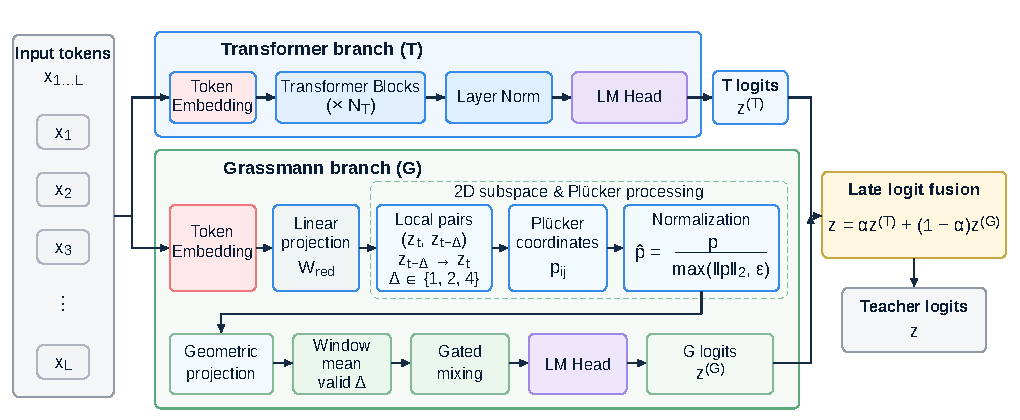
\includegraphics[width=\textwidth]{figures/figA1_teacher_architecture.pdf}
\caption{通用异构教师模型。Grassmann 路径使用因果局部词元对、归一化 Pl\"ucker 坐标、几何投影、有效窗口平均、门控混合及 LM head。后融合在 logits 上进行，$\alpha$ 为自由参数。该架构不能证明几何 KD 的优越性。}
\label{fig:teacher_architecture}
\end{figure*}

\section{训练协议与重要修订}\label{app:protocols}

\subsection{语料与匹配学生模型}
PTB 和 WikiText-2 使用归档的原始划分；TinyStories 使用种子 42 将训练数据按 98/2 划分，并将原始验证集用作测试集。PTB 包含 42,068 个非空训练文本行和 4,439 个训练数据块。TinyStories 使用 300,000 个训练文本行（截断前 67,081,279 个词元；262,036 个数据块）、42,391 个验证文本行（9,440,302 个词元；36,876 个数据块）和 21,990 个测试文本行（4,765,822 个词元；18,616 个数据块）。固定长度为 256 个词元的数据块在评估时使用位置 1--255；留出集的目标词元不进入训练。

每个主要实验种子独立训练自己的 $S_0$，使用 20 轮训练、批大小 32、学习率 $2\times10^{-4}$、权重衰减 0.01、AMP，并按验证集 NLL 选择检查点。初始训练使用 AdamW、源实现的默认配置和固定学习率。续训重新初始化 AdamW，使用 10 轮训练、批大小 32、学习率 $10^{-4}$、权重衰减 0.01、5\% 线性预热后接余弦衰减、AMP、裁剪阈值 1 和 $\tau=2$。CE（0）与 KD（5）之间仅 $\lambda$ 不同。前向 KL 对有效目标词元取平均，并包含温度平方缩放。这些配置在本轮论文修改前已经冻结。

共同的 WikiText-2 子集包含 512 个验证数据块，使用种子 20260920 无放回抽样后排序（130,560 个目标词元）。完整验证集上的 TT/TG 指标保持单独报告。J 在该子集上的重复评估值 4.300644 和 4.300646 保留原始精度，不合并取平均。

\subsection{教师模型训练与准入条件}
PTB 和 TinyStories 的教师模型均将宽度为 256 的六层 Transformer 与宽度为 240、降维宽度为 64、时间间隔为 $\{1,2,4\}$ 的六层 Grassmann 分支组合；两个分支均使用 dropout 0.1。源模型训练使用种子 42、20 轮训练、批大小 32、序列长度 256 和学习率 $3\times10^{-4}$；四个源模型均按验证集选择第 20 轮。融合教师模型联合训练十轮，在第 1 轮冻结分支，使用分支学习率 $10^{-5}$、权重衰减 0.01、AMP、初始 $\alpha=0.5$ 和 late-$k=1$。两者的融合权重学习率分别为 $5\times10^{-3}$ 和 $10^{-2}$。验证集分别选择融合模型的第 8 和第 10 轮；主要续训保留学得的 $\alpha=0.470293$ 和 $0.599406$，而强制 $\alpha=0.5$ 适用于 WikiText-2 对照。

表~\ref{tab:teacher_training_protocol} 记录了教师模型的训练模式。J 和 TT 联合训练十轮；A 仅训练融合权重五轮。状态干预固定部署时的架构与组成，而不固定教师模型的训练历史。TT 的源 Transformer 具有六层网络、宽度 256、dropout 0.1、批大小 32、学习率 $3\times10^{-4}$ 和 20 轮训练，使用种子 42 和 123；两者均选择第 12 轮。TT 联合训练选择第 10 轮。其融合学习率与历史 TG 配置不同。
\begin{table*}[!t]\centering
\begin{tabular}{llrrr}
\toprule
教师模型 & 模式 & 训练轮次预算 & 分支学习率 & 融合权重学习率\\
\midrule
J/TG & 联合训练 & 10 & $10^{-5}$ & $5\times10^{-3}$\\
A & 仅训练融合权重 & 5 & 冻结 & $10^{-2}$\\
TT & 联合训练 & 10 & $10^{-5}$ & $10^{-2}$\\
\bottomrule
\end{tabular}
\caption{归档的 WikiText-2 教师模型训练配置。所有模型均以 $\alpha=0.5$ 初始化，使用批大小 32、权重衰减 0.01 和 AMP，并按验证集选择检查点。联合训练分支在第 1 轮冻结；A 全程冻结分支。评估和 KD 均强制 $\alpha=0.5$。这些训练历史不能单独识别教师模型的标量质量或架构效应。}
\label{tab:teacher_training_protocol}
\end{table*}


联合训练改变了 179 个 J/A 状态张量，全部状态张量共计 191 个。缩减数据的准入 smoke test 中，裁剪比例为 1，AMP/非有限值比例为 0.16。经授权，以全量数据进行的一轮训练准入检查替代了该测试，目标函数与裁剪阈值均未改变。J/A 准入检查的裁剪比例为 0.234694 和 0.275510，两者的 AMP/非有限值比例均为 0.013605。A/J 参数梯度比 1.102792、1.148522 和 1.093056 均满足预注册区间 $[0.5,2]$。A 正式训练第一轮的裁剪比例为 0.666667、0.503401 和 0.513605；AMP/非有限值比例的最大值为 0.013605。

T-only 需要单独授权的准入条件修订：全量数据准入检查中每次更新均触发裁剪，但参数梯度保持有限，T/F 比为 1.3164、1.2788 和 1.2324，AMP/非有限值比例为 0.013605。正式训练保留了全部配置。第一轮仍完全裁剪饱和；各轮次的平均裁剪比例为 0.4990、0.4605 和 0.4398，在训练后期降至约 0.0034。三个种子均选择第 10 轮。永久保留的 \texttt{CLIP\_SATURATION\_WARNING} 限制了对 F--T 差距的解释。

TT 学生模型第一轮的裁剪比例为 0.928571、0.843537 和 0.874150；对应的跨训练轮次均值为 0.170068、0.137755 和 0.127551。AMP/非有限值比例的最大值为 0.013605。这些轨迹与 TG 并非严格的优化匹配。

\subsection{TinyStories 稳定性与接受的重试}
主要 TinyStories 实验的所有 CE 和 KD 分支均选择第 10 轮。各种子的 CE 平均裁剪比例均为 0.000391；KD 均值为 0.236891、0.283344 和 0.240090（表~\ref{tab:tinystories_optimization}）。AMP/非有限值比例的最大值在 CE 中为 0.000488，在 KD 中为 0.000611。接受的终点指标均有限，KD 并未持续完全裁剪饱和。

种子 456 的一次运行因基础设施功率限制在第 2 轮中断，并在产生任何最终终点前被排除。经授权完成的重试从相同 $S_0$ 重新开始，使用新优化器，并保持教师模型、种子、数据、目标函数、预算和选择规则不变。只有完成的重试计入结果。实验使用 RTX 3090 GPU；详细的总体计算资源统计不可用，本文不对此进行推断。
\begin{table}[!t]\centering
\begin{tabular}{lrrrrr}
\toprule
种子 & 残余优势 & KD KL & CE 范数 & KD 范数 & KD 裁剪比例 \\
\midrule
42 & -0.021960 & 0.380224 & 0.486891 & 0.973546 & 0.236891 \\
123 & -0.021422 & 0.381402 & 0.488263 & 0.981438 & 0.283344 \\
456 & -0.019714 & 0.383282 & 0.483211 & 0.973942 & 0.240090 \\
\bottomrule
\end{tabular}
\caption{主要 TinyStories 实验的训练监测指标。残余优势为教师模型相对于 CE 测试集终点的优势。KL 包含温度平方缩放；范数和裁剪比例为已完成运行各训练轮次的均值。}\label{tab:tinystories_optimization}
\end{table}


\section{完整逐种子结果}\label{app:per-seed}

\begin{table*}[!t]\centering
\begin{tabular}{lrrr}
\toprule
条件 & 种子 42 & 种子 123 & 种子 456 \\
\midrule
PTB 融合 & 0.142284 & 0.149462 & 0.143066 \\
TinyStories 融合 & -0.107479 & -0.107439 & -0.106740 \\
WT2 J/TG & 0.162501 & 0.147337 & 0.157157 \\
WT2 A & -0.022394 & -0.035362 & -0.025206 \\
WT2 G & 0.046771 & 0.033598 & 0.042604 \\
WT2 T & 0.142785 & 0.125226 & 0.136593 \\
WT2 TT & 0.176453 & 0.158666 & 0.169257 \\
\bottomrule
\end{tabular}
\caption{归档的配对测试集 NLL 增益。正值表示 KD 更优；同一种子内的所有 WikiText-2 分支共用相同的 CE 终点。}\label{tab:per_seed_gains}
\end{table*}


表~\ref{tab:per_seed_gains} 给出了确认性实验各组的配对测试集增益。增益根据归档的 NLL 计算，而非对四舍五入后的 PPL 取对数。同一种子内的所有 WikiText-2 分支共用其 CE 对照，J/TG 是同一个复用终点。CE/KD 测试集 NLL 均值分别为 4.082352/3.937415（PTB）、4.276364/4.120699（WikiText-2）和 1.582197/1.689416（TinyStories）。表~\ref{tab:ptb_endpoints}、\ref{tab:wt2_endpoints} 和~\ref{tab:ts_endpoints} 报告了所选终点。
\begin{table}[!t]\centering
\begin{tabular}{lrrrrrr}
\toprule
种子 & CE 测试 & KD 测试 & CE 验证 & KD 验证 & CE 轮次 & KD 轮次 \\
\midrule
42 & 4.079528 & 3.937244 & 4.237272 & 4.081793 & 1 & 10 \\
123 & 4.088605 & 3.939143 & 4.243102 & 4.082198 & 1 & 10 \\
456 & 4.078925 & 3.935859 & 4.244354 & 4.082000 & 1 & 9 \\
\bottomrule
\end{tabular}
\caption{归档的所选检查点汇总中的 PTB 测试集与验证集 NLL。配对差值与确认性结果清单一致；各分支独立按验证集选择训练轮次。}\label{tab:ptb_endpoints}
\end{table}

\begin{table}[!t]\centering
\begin{tabular}{lrrrrrr}
\toprule
种子 & CE & KD(J/TG) & KD(T) & KD(G) & KD(A) & KD(TT) \\
\midrule
42 & 4.270742 & 4.108241 & 4.127957 & 4.223972 & 4.293136 & 4.094289 \\
123 & 4.277520 & 4.130183 & 4.152294 & 4.243922 & 4.312882 & 4.118854 \\
456 & 4.280830 & 4.123673 & 4.144237 & 4.238226 & 4.306036 & 4.111574 \\
\bottomrule
\end{tabular}
\caption{WikiText-2 所选学生模型的测试集 NLL。J/TG 是同一个复用的融合终点，而非两个实验。所有 KD 列均报告学生模型终点，而非教师模型似然。}\label{tab:wt2_endpoints}
\end{table}

\begin{table*}[!t]
\centering
\begin{tabular}{lrrrr}
\toprule
种子 & $S_0$ 测试 & CE 测试 & KD 测试 & 验证集 KD--CE\\
\midrule
42 & 1.622437 & 1.581269 & 1.688747 & 0.108394\\
123 & 1.623954 & 1.581807 & 1.689246 & 0.108082\\
456 & 1.624901 & 1.583515 & 1.690255 & 0.108040\\
\bottomrule
\end{tabular}
\caption{TinyStories 所选 NLL。所有分支均选择第 10 轮。正的验证集 KD--CE 差值与负的 CE 相对测试集增益方向一致。}
\label{tab:ts_endpoints}
\end{table*}


在共同子集上，G 教师模型相对于验证集所选 CE 终点的残余优势为 $-0.266520$、$-0.253492$ 和 $-0.251006$，而测试集增益为 $+0.046771$、$+0.033598$ 和 $+0.042604$。参照对象是 CE，而非 $S_0$。教师模型似然与增益对应不同的留出集范围；这些种子并未独立重复教师模型训练。

教师模型状态对比量 $Q$ 分别为 0.184895、0.182699 和 0.182364，对应种子 42、123 和 456，均值为 $0.183319\pm0.001375$。监督源的均值与样本标准差分别为 F $0.155665\pm0.007692$、T $0.134868\pm0.008906$ 和 G $0.040991\pm0.006733$。F--T 与 F--G 差值分别为 $0.020797\pm0.001214$ 和 $0.114674\pm0.001001$。教师监督源的子集 NLL 为 4.300646、4.445647 和 4.652064。组成变化也会改变预测质量。

在完整验证集上，TG/TT 教师模型 NLL 为 4.303697/\allowbreak4.293589；TG 的分支 NLL 为 4.451680/\allowbreak4.655020，TT 为 4.406160/\allowbreak4.422151。TG 的参数量为 37,749,633，TT 为 35,340,801。两者的 KD 增益为 $0.155665\pm0.007692$ 和 $0.168125\pm0.008948$。配对 $H$ 的均值为 $-0.012460\pm0.001348$，三个种子均为负值。表~\ref{tab:branch_comparison} 将完整验证集分支指标与子集干预指标分开报告。更高的 TG 分支分歧度并未产生更好的迁移，但质量、参数量和训练历史的混杂因素使该对比不能用于架构或分歧度的因果判断。
\begin{table}[!t]
\centering
\begin{tabular}{lrrrr}
\toprule
教师模型 & 完整验证集 NLL & 分支 JSD & 一致率 & 融合增益\\
\midrule
TG & 4.303697 & 0.182087 & 0.507034 & 0.147983\\
TT & 4.293589 & 0.099793 & 0.630170 & 0.112570\\
\bottomrule
\end{tabular}
\caption{$\alpha=0.5$ 时完整验证集上的教师模型对比。融合增益为相对于较优分支的 NLL 改善。预测质量、参数量和训练历史均不同。这些指标不与 512 个数据块的状态/监督源子集指标合并。}
\label{tab:branch_comparison}
\end{table}


\section{诊断与现代模型压力测试细节}\label{app:diagnostics-modern}

\subsection{分支分歧与回顾性探测}
在共同验证子集上，J 的分支 NLL 分别为 4.445648 和 4.652064，JSD 为 0.181288，预测一致率为 0.508395，相对于较好分支的融合增益为 0.145003。A 的分支 NLL 分别为 6.540640 和 6.696787，JSD 为 0.176641，预测一致率为 0.543719，融合增益为 0.164420。质量发生了较大变化，但分歧或融合增益并未出现一致有利的变化。

词元级分歧分析对每个语料仅使用一组经选择的 CE/KD 模型对，并非三个模型重复实验。在 CE 词元难度之外加入 JSD 后，梯度冲突 AUROC 的增量在 PTB 上为 $-0.000323$，在 TinyStories 上为 $+0.010910$；最终结果 $R^2$ 的增量分别为 $+0.000533$ 和 $+0.003061$。词元/分块 bootstrap 不确定性并不会产生独立的模型种子。这些微小增量不能确立分歧是一种强迁移机制。

局部诊断指标覆盖七个组合及 21 个存在依赖关系的种子级条件。训练探测使用前 32 个分块，以 FP32、大小为二的微批遍历全部学生参数。校准种子 314159、271828 和 161803 各选取两个不重叠的验证分块，共得到 63 行结果。评分在合并最终结果前冻结；探测未使用测试数据，也未保留任何参数更新。

在 $S_0$ 处，令 $g=\nabla\mathcal L_{\mathrm{CE}}$、$k=\nabla\mathcal L_{\mathrm{distill}}$、$v=\nabla\mathcal L_{\mathrm{val}}$ 及 $H_{\mathrm{val}}=\nabla^2\mathcal L_{\mathrm{val}}$。定义 $a=v^\top k$、$b=g^\top H_{\mathrm{val}}k$ 及 $c=k^\top H_{\mathrm{val}}k$。名义 Taylor 诊断为
\begin{equation}
\widehat G_{\mathrm{local}}(\lambda)=\eta\lambda a-\eta^2\lambda b-\tfrac12\eta^2\lambda^2c,
\end{equation}
其中 $\eta=10^{-4}$。它并不是所选测试集最终结果的界。全部梯度与 HVP 均为有限值；一阶/二阶符号在 63/63 行中一致，种子级 AUROC 为 0.644444，符号准确率为 0.571429，组合均值 AUROC 为 0.600000。两者均未正确识别具有正向结果的 WikiText-2 J、G 及 TT 组合。仅 11/21 个条件的符号在不同校准子集间保持稳定。曲率修正绝对值的中位数为 $2.73\times10^{-7}$（为一阶量级的 0.52\%），且从未改变符号。

实际调度的第一步学习率为零，不产生更新，因此不能视为安全性结果。一个使用名义学习率并进行裁剪的 AdamW 虚拟诊断，其 AUROC 为 0.700000，准确率为 0.571429；它未正确识别 9/15 个有益结果，仅在 10/21 个条件上具有稳定符号。表~\ref{tab:full_predictors} 报告了合并的回顾性评分。结果间的依赖关系与有限的覆盖范围，使其无法确立普遍选择规则，也不能用于与自适应方法比较。
\begin{table}[!t]\centering
\begin{tabular}{lrrr}
\toprule
预测量 & AUROC & 符号准确率 & $\rho$ \\
\midrule
教师模型残余优势 & 0.711111 & 0.523810 & 0.437662 \\
教师模型验证集 NLL & 0.500000 & -- & 0.235921 \\
KL 大小 & 0.722222 & -- & 0.450649 \\
KD 梯度范数 & 0.500000 & -- & -0.118182 \\
训练集 CE-KD 余弦 & 0.477778 & 0.714286 & -0.024675 \\
验证集点积 a & 0.644444 & 0.571429 & 0.249351 \\
验证集余弦 & 0.644444 & 0.571429 & 0.285714 \\
二次增益 & 0.644444 & 0.571429 & 0.249351 \\
虚拟名义增益 & 0.700000 & 0.571429 & 0.427273 \\
\bottomrule
\end{tabular}
\caption{21 个相互依赖条件上的完整种子级回顾性预测量对比。横线表示该预测量未定义此指标，而非数值为零。}\label{tab:full_predictors}
\end{table}


\subsection{现代模型续训与检查点候选资格}
SmolLM2 学生/教师基座模型的参数量分别为 134,515,008/361,821,120，共享词表大小为 49,152。360M 教师模型适配一次后即被冻结。学生种子分别独立适配同一个预训练的 135M 基座，并非使用独立预训练的模型。FP32 权重使用 BF16 自动混合精度与 FP32 损失，不使用 GradScaler。AdamW 的学习率为 $5\times10^{-5}$，权重衰减为 0.01，betas 为 $(0.9,0.95)$，epsilon 为 $10^{-8}$，使用 5\% 预热与余弦衰减。序列长度为 256，批大小为 32，微批大小为 4，裁剪阈值为 1，且 $\tau=2$。教师适配、学生准备及续训各使用 10M 个目标词元（1,221 次更新）。

FineWeb-Edu 使用 \texttt{sample-10BT} 的分片 \texttt{sample/10BT/000\_00000.parquet}，修订版本为 \texttt{87f09149ef4734204d70e}\allowbreak\texttt{d1d046ddc9ca3f2b8f9}。确定性的文档 ID 哈希及精确文本去重得到相互不重叠的训练、验证和测试划分，分别包含 20M、1M 和 1M 个编码后的词元；每个留出集评估 999,999 个目标。主要验证候选为第 256、512、768、1024 和 1221 步，不包含 $S_0$。测试集评估在选择之后进行。表~\ref{tab:modern_endpoints} 报告这些最终结果；表~\ref{tab:modern_optimization} 给出所选步数及记录的遥测指标。

教师模型的验证/测试 NLL 为 2.747486/\allowbreak2.726017，优于每个 $S_0$。然而，CE 测试 NLL 相较于 $S_0$ 分别增加了 0.005562、0.005268 和 0.012924（均值为 $+0.007918\pm0.004338$）。允许第 0 步参与选择后，全部九个 CE/KD 训练臂均选择 $S_0$，诊断性的 CE 相对增益为零。这不会替代以训练后检查点为候选的主要比较。确切的预训练重叠仍未知。
\begin{table*}[!t]\centering
\begin{tabular}{lrrrrr}
\toprule
种子 & 划分 & $S_0$ & CE & KD1 & KD5 \\
\midrule
42 & 验证集 & 2.967112 & 2.973155 & 2.988861 & 3.019882 \\
42 & 测试集 & 2.944338 & 2.949900 & 2.965619 & 2.996304 \\
123 & 验证集 & 2.967390 & 2.973067 & 2.988537 & 3.019533 \\
123 & 测试集 & 2.944865 & 2.950133 & 2.965603 & 2.996212 \\
456 & 验证集 & 2.967554 & 2.980508 & 2.990422 & 3.020545 \\
456 & 测试集 & 2.944959 & 2.957883 & 2.967346 & 2.997173 \\
\bottomrule
\end{tabular}
\caption{冻结的 FineWeb-Edu 主要终点。CE/KD 的验证集选择排除第 0 步。仅在该选择完成后评估测试集；单独的 best-including-S0 诊断在全部九个分支中均选择 S0。}\label{tab:modern_endpoints}
\end{table*}

\begin{table*}[!t]\centering
\begin{tabular}{lrrrrr}
\toprule
种子 & 分支 & 步数 & 裁剪比例 & 平均范数 & 最大范数 \\
\midrule
42 & S0 & 256 & 0.129402 & 0.947446 & 3.142341 \\
42 & CE & 1221 & 0.058968 & 0.929848 & 1.394476 \\
42 & KD1 & 1221 & 0.850123 & 1.084600 & 2.502529 \\
42 & KD5 & 1221 & 1.000000 & 2.557157 & 11.615945 \\
123 & S0 & 256 & 0.117117 & 0.948927 & 4.028796 \\
123 & CE & 1221 & 0.056511 & 0.929663 & 1.203820 \\
123 & KD1 & 1221 & 0.854218 & 1.090724 & 3.144516 \\
123 & KD5 & 1221 & 1.000000 & 2.601404 & 19.092007 \\
456 & S0 & 1221 & 0.127764 & 0.944769 & 1.363758 \\
456 & CE & 256 & 0.045045 & 0.994147 & 86.482155 \\
456 & KD1 & 1221 & 0.798526 & 1.074831 & 2.708021 \\
456 & KD5 & 1221 & 1.000000 & 2.545350 & 12.600890 \\
\bottomrule
\end{tabular}
\caption{FineWeb-Edu 优化审计。步数按验证集在已训练检查点中选择。范数均在裁剪前测量；所有已记录的非有限值和溢出比例均为零。}\label{tab:modern_optimization}
\end{table*}


初始未加权 KD/CE 梯度比为 2.150561、2.485828 和 2.462981。KD1 的裁剪比例为 0.850123、0.854218 和 0.798526；KD5 每次更新均触发裁剪。记录到的溢出/非有限值比例均为零。KD5 保留 \texttt{CLIP\_SATURATION\_WARNING}。种子 456 的 CE 在第 711 步、即其所选第 256 步之后，裁剪前梯度范数达到 86.482155。该尖峰的原因及其对轨迹的影响未知；该运行仍被纳入结果，并保留 \texttt{CE456\_GRADIENT\_SPIKE\_WARNING}。

\subsection{未通过的不重叠续训改进空间门控}
仅使用 CE 的对照固定采用种子 42 的准备阶段第 256 步检查点，此时已经使用 2,097,152 个目标，而不是按验证结果选择 $S_0$。冻结清单排除已消耗的 8,192 个目标分块，并提供 31,250 个新分块（8M 个目标）。边界上下文可能共享，但预测目标已被排除。清单与顺序均在观察到续训最终结果前固定。

候选学习率 $5\times10^{-6}$、$10^{-5}$ 和 $2\times10^{-5}$ 保持优化器类别、调度器、批大小、序列长度、裁剪及预算不变。验证选择包含第 0、256、512、768 和 977 步，同值时选择较早的检查点。全部候选均选择第 977 步。改进分别为 0.004214、0.004849 和 0.003941，均低于 0.01 门槛（表~\ref{tab:modern_ce_gate}）；裁剪比例为 0.060389、0.079836 和 0.082907，非有限值比例为零。最高学习率的训练臂在第 656 步出现了有限的梯度范数尖峰 14.602655，其原因与影响未知。

冻结的决策为
\texttt{STOP\_}\allowbreak\texttt{MODERN\_}\allowbreak\texttt{CONTINUATION\_}\allowbreak\texttt{NOT\_}\allowbreak\texttt{ESTABLISHED}。
没有测量以门槛通过为前提的 $\lambda=0.25$ 或 1 的 KD、新的测试集最终结果及初始 KD/CE 梯度比。这些量是按设计未测量，而不是零。该压力测试不能证明 FineWeb-Edu 导致负迁移、较好的教师模型通常会损害 KD，或所有现代模型 KD 均会失败。
\begin{table}[!t]
\centering
\begin{tabular}{lrrrr}
\toprule
CE 峰值学习率 & 所选验证集 NLL & 验证集改善 & 所选步数 & 准入结果 \\
\midrule
5e-06 & 2.962897 & 0.004214 & 977 & 未通过 \\
1e-05 & 2.962263 & 0.004849 & 977 & 未通过 \\
2e-05 & 2.963171 & 0.003941 & 977 & 未通过 \\
\bottomrule
\end{tabular}
\caption{从固定的早期 $S_0$ 开始、仅使用 CE 的不重叠续训准入检查，种子为 42。验证集选择包含第 0 步。所有候选学习率均未达到要求的 0.01 改善，因此未执行条件性 KD 或新的测试集评估。}
\label{tab:modern_ce_gate}
\end{table}


\FloatBarrier
\section*{归档说明}
说明：本中文版仅用于课题组内部留档与报备。正式投稿版本为英文版 COLING 2027 / ACL Rolling Review 稿件。如中英文表述存在差异，以最终英文投稿稿为准。
\end{document}
